\pdfminorversion=4
\documentclass[aspectratio=169,hyperref={unicode},notheorems]{beamer}


\mode<presentation>
{
  \usetheme{default}
  \usecolortheme{default}
  \usefonttheme{default}
  \setbeamertemplate{navigation symbols}{}
  \setbeamertemplate{caption}[numbered]
  \setbeamertemplate{footline}[frame number]  % or "page number"
  \setbeamercolor{frametitle}{fg=white}
  \setbeamercolor{footline}{fg=black}
} 

\usepackage[T2A]{fontenc}
\usepackage[utf8]{inputenc}
\usepackage[russian]{babel}
\usepackage{tikz}
\usepackage{courier}
\usepackage{array}
\usepackage{bold-extra}
\usepackage{minted}
\usepackage[thicklines]{cancel}
\usepackage{fancyvrb}

\xdefinecolor{dianablue}{rgb}{0.18,0.24,0.31}
\xdefinecolor{miptdeepblue}{RGB}{0,94,184}
%\xdefinecolor{darkblue}{rgb}{0.1,0.1,0.7}
%\xdefinecolor{darkgreen}{rgb}{0,0.5,0}
\xdefinecolor{darkgrey}{rgb}{0.35,0.35,0.35}
%\xdefinecolor{darkorange}{rgb}{0.8,0.5,0}
%\xdefinecolor{darkred}{rgb}{0.7,0,0}
%\definecolor{darkgreen}{rgb}{0,0.6,0}
%\definecolor{mauve}{rgb}{0.58,0,0.82}

\title[2019-06-25-Защита диссертации на степень бакалавра]{Спектры предложений первого порядка с ограниченным количеством переменных}
\author{Ярмошик Демьян}
\institute{Московский физико-технический институт (НИУ)}
\date{25 июня, 2019}

\usetikzlibrary{shapes.callouts}
\usetikzlibrary{decorations.pathmorphing}
\usepackage{ mathrsfs }
\usepackage{ dsfont }
\newtheorem {theorem}{Теорема}
\theoremstyle{definition}
\newtheorem {definition}{Определение}
\def \LL     {\mathcal{L}}
\def \N    {\mathbb {N}}
\def \F   {\mathcal{F}}
\def \R    {\mathbb {R}}
\def \Q    {\mathbb {Q}}
\def \P {{\sf P}}
\def \E {\mathds{E}}
\def \eps {\varepsilon}
\def \Gna {G\left(N,N^{-\alpha}\right)}
\def \bfN {\mathbf{N}}

\begin{document}

\logo{\pgfputat{\pgfxy(0.11, 7.4)}{\pgfbox[right,base]{\tikz{\filldraw[fill=miptdeepblue, draw=none] (0 cm, 0 cm) rectangle (50 cm, 1 cm);}\mbox{\hspace{-8 cm}
\includegraphics[height=1cm]{brandbook/mipt-inversed-transparent.png}
\includegraphics[height=1cm]{brandbook/fpmi-inversed-transparent-smaller.png}}}}}

\begin{frame}
\setbeamercolor{title}{fg=miptdeepblue}
  \titlepage
\end{frame}

\logo{\pgfputat{\pgfxy(0.11, 7.4)}{\pgfbox[right,base]{\tikz{\filldraw[fill=dianablue, draw=none] (0 cm, 0 cm) rectangle (50 cm, 1 cm);}\mbox{\hspace{-8 cm}
\includegraphics[height=1 cm]{brandbook/mipt-logo.png}
\includegraphics[height=1 cm]{brandbook/fpmi-logo-spaces.png}}}}}

% Uncomment these lines for an automatically generated outline.
%\begin{frame}{Outline}
%  \tableofcontents
%\end{frame}

% START START START START START START START START START START START START START
%-2----------------------------
\begin{frame}{Модель Эрдёша--Реньи}
\vspace{0.5 cm}
Случайный граф $G(N, p) \in \Omega_N,~|\Omega_N|=2^{C_N^2}$

$\P: 2^{\Omega_N} \rightarrow [0,1]$
\vspace{0.5 cm}

\[\P_{N,p}(G) = p^{|E|}(1-p)^{C_N^2-|E|}\]

Обычно $p = p(N) = N^{-\alpha}$
\end{frame}
%-3----------------------------
\begin{frame}{Эволюция $G(N,p)$}
%\vspace{0.5 cm}
\begin{figure}
\tikz[scale=0.9, every node/.style={scale=0.9}]{
\draw[thick] (-1,0) -- (12,0);
    \draw (-1, 1.5) node {пустой};
    \draw (6, 1.5) node {разреженный};
    \draw (11.5, 1.5) node {плотный};
    \draw (0, 0.8) node {$N^{-2}$}; \draw (0,0.5) -- (0, -0.5);
    \draw (5, 0.8) node {$N^{-\frac{3}{2}}$}; \draw (5, 0.4) -- (5, -0.4);
    \draw (7.5, 0.8) node {$N^{-\frac{4}{3}}$}; \draw (7.5,0.3) -- (7.5, -0.3);
     \draw (8.75,0.8) node {$N^{-\frac{5}{4}}$}; \draw (8.75,0.2) -- (8.75, -0.2); %\draw (4.8,0.18) -- (4.8, -0.18);
    \draw (10, 0.8) node {$N^{-1}$}; \draw (10,0.5) -- (10, -0.5);
\draw[thick] (-1, -3) -- (5.5, -3);
\draw[thick, dashed] (5.5, -3) -- (7.5, -3);
\draw[thick] (7.5, -3) -- (12, -3);
    \draw (3,-2.5) -- (3, -3.5);
    \draw (10,-2.5) -- (10, -3.5);
    \draw (1,-2) node {$\dfrac{c}{N},~ c < 1$};
    \draw (3,-2) node {$\dfrac{1}{N}$};
    \draw (5,-2) node {$\dfrac{c}{N},~ c > 1$};
    \draw (8,-2) node {$\dfrac{c\ln{N}}{N},~ c < 1$};
    \draw (10,-2) node {$\dfrac{\ln{N}}{N}$};
    \draw (12,-2) node {$\dfrac{c\ln{N}}{N},~ c > 1$};
}
 %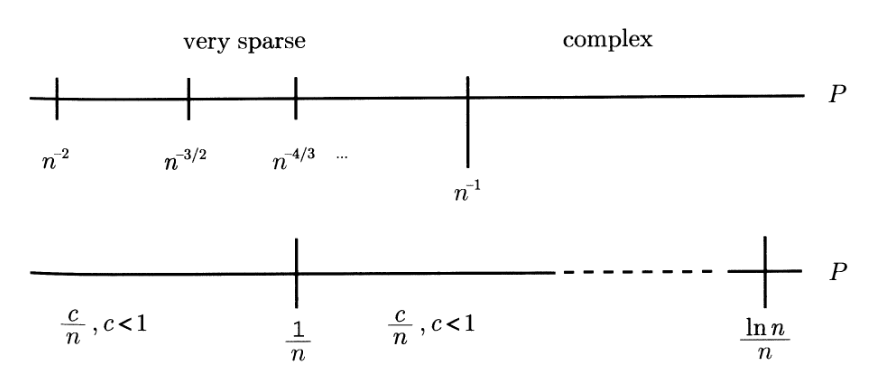
\includegraphics[scale=0.3]{picrel/evolution.png}
  %\caption{Несколько блоков и дополнительное ребро}
\end{figure}
\end{frame}
%-4----------------------------
\begin{frame}{Теоремы о вхождении подграфа}
\vspace{0.5 cm}
\begin{theorem}[А. Ручински, А. Винс, 1985] 
\label{th:ruchinski}
Функция $N^{-1/\rho^{max}(H)}$ является пороговой для случайного графа $G(N,p)$ и свойства содержать копию графа $H$ в качестве подграфа.
\end{theorem}
\begin{theorem} [Б. Боллобаш, 1981] 
Пусть $H$~--- строго сбалансированный граф, $a$~--- количество автоморфизмов графа $H$, $p = N^{-1/ \rho^{max}(H)}$.
Тогда
\[N_H \xrightarrow[N\rightarrow \infty]{d} Poiss(1/a). \]
Здесь $N_H$~--- количество копий графа $H$ в $G(N, p)$, $Poiss(1/a)$~--- пуассоновская случайная величина со средним $1/a$.
\end{theorem}
\end{frame}
%-5----------------------------
\begin{frame}{Языки первого порядка на графах}
\vspace{0.5 cm}
Язык первого порядка $\LL$:

переменныe: $x,y,z,x_1,x_2\ldots$; 

логическиe связки: $\wedge, ~\neg, ~\vee$; 

кванторы по переменным: $\exists x, ~\forall z$;

предикатные символы: $\sim, ~ =$.

\[ \forall x~ \exists y \exists z~ (x\sim y \wedge x\sim z \wedge y \sim z) \]

\end{frame}

%-6----------------------------
\begin{frame}{Закон нуля или единицы}
\vspace{0.5 cm}
\begin{definition}
    Для произвольного языка $\F$, случайный граф $G(N, p)$ \textit{подчиняется закону нуля или единицы для языка $\F$},
    если для любой формулы $\varphi$ из языка 
    $\F$  выполнено
\[\lim_{N \rightarrow \infty} \P(G(N, p) \vDash \varphi) \in \{0, 1\}.\]
\end{definition}
\begin{theorem} [Дж. Спенсер, С. Шелах, 1988]
Случайный граф $G(N, N^{-\alpha})$ подчиняется закону нуля или единицы для языка $\LL$ при всех $\alpha$, кроме 
\[\left((0,1] \cap \Q \right) \cup \{(k+1)/k ~|~ k \in \N \}.\]
\end{theorem}
\end{frame}
%-7----------------------------
\begin{frame}{Языки $\LL^k$, $\LL^k_{\infty, \omega}$}
\begin{definition}
    Язык $\LL^k$~--- подмножество $\LL$, содержащее предложения, в которые входят не более $k$ переменных.
\end{definition}
В $\LL^3$ можно выразить свойство ``иметь диаметр не более d'':
\[
\psi_d = \forall x \forall y ~ x = y \vee x \sim y \vee \left( \exists z ~ x\sim z \wedge z \sim y \right)
\vee  \left( \exists z ~ x\sim z \wedge \left( \exists x ~ z \sim x \wedge x \sim y \right) \right) \vee \ldots
\]
\begin{definition}
    Язык $\LL^k_{\infty, \omega}$ включает в себя предложения конечной или счётной длины, в которые входят не более $k$ переменных.
\end{definition}
\end{frame}

%-----------------------------------------
\begin{frame}{Постановка задачи}
\begin{definition}
    \textit{Спектром} формулы $\varphi$ называется множество $\alpha$ таких, что вероятность $\P\left( G\left(N, N^{-\alpha}\right) \vDash \varphi  \right)$ не стремится ни к 0, ни к 1 при $N \rightarrow \infty$.
\end{definition}
\vspace{0.5 cm}
    \begin{itemize}
        \item Нарушется ли закон нуля или единицы для $\LL^3,~ \LL^3_{\infty, \omega}$ в окрестности 1?
        \item Отличается ли структура спектров формул этих языков от спектров формул языка $\LL$ и языков с ограниченной кванторной глубиной?
    \end{itemize}
\end{frame}

%-----------------------------------------
\begin{frame}{Методы}
\begin{itemize}
    \item Теоремы о вхождении подграфа
    \item Игра Эренфойхта и модификации: k-Pebble и др.
\end{itemize}
\end{frame}

%-----------------------------------------
\begin{frame}{Сравнение спектров в правой окрестности единицы }
\vspace{0.5 cm}
В $\LL$ в правой полуокрестности единицы закон нуля нарушается в точках $\dfrac{k+1}{k}$.
\vspace{0.5 cm}

Доказано: в $\LL^3_{\infty, \omega}$ есть формула $\varphi$, у которой в точках $\alpha = \dfrac{k+1}{k}$ вероятность $\P(\Gna \vDash \varphi)$ имеет предел, отличный от 0 и 1.
\end{frame}

% %---------------------------------------
% \begin{frame}{Левая окрестность единицы: $\alpha \in \Q$}

% \vspace{0.5 cm}

% О спектрах предложений $\LL^3,~\LL^3_{\infty, \omega}$ в интервале $\left( \dfrac{1}{2}, 1\right)$ ничего не знали.
% \end{frame}

%---------------------------------------
\begin{frame}{Левая окрестность единицы: $\alpha \in \Q$}
\begin{theorem}
Объединение спектров всех формул из $\LL^3$ имеет предельные точки в любой левой окрестности единицы.
\end{theorem}
\begin{figure}
    \centering
    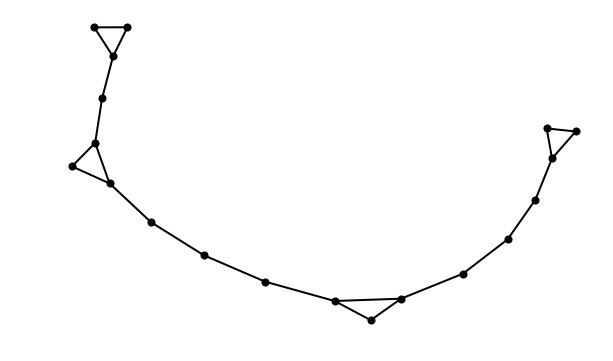
\includegraphics[scale=0.3]{picrel/Hksm.png}
\end{figure}
\end{frame}

%------------------------------------------
\begin{frame}{Левая окрестность единицы: $\alpha \in (\frac{1}{2},1) \setminus \Q$}

\begin{definition}
    \[\LL^\omega_{ \infty,\omega} = \bigcup_{k=1}^\infty \LL^k_{ \infty,\omega}\]
\end{definition}

\begin{theorem}[С. Шелах, 2017]
$\Gna$ не подчиняется закону нуля или единицы для языка $\LL^\omega_{ \infty,\omega}$ при $\alpha \in (0, 1]$.
\end{theorem}

\visible<2>{
\begin{itemize}
    \item Большие $k$.
    \item До сих пор нет публикации.
    \item Сложное решение.
\end{itemize}
}
\end{frame}


%--------------------------------------------
\begin{frame}{Левая окрестность единицы: $\alpha \in (\frac{1}{2},1) \setminus \Q$}
\begin{figure}
    %\centering
    \includegraphics<1>[scale=0.4]{picrel/1_block_tall.png}
    \includegraphics<2>[scale=0.4]{picrel/2_blocks_tall.png}
    \includegraphics<3->[scale=0.4]{picrel/2_blocks+.png}
\end{figure}
\visible<4>{
\begin{figure}
    \centering
\tikz[scale=0.75, every node/.style={scale=0.5}] {
    \draw (-1.5, 0) node {$v^{max}$};
    \draw (-0.5,0) --  (14,0);
        \draw (0,0) node {\textbf[ };
            \draw (0, 0.5) node {$v_1$};
        \draw (3,0) node {\textbf] };
            \draw (3.3, 0.5) node {$10\bfN_{v_1}$};
        \draw (5,0) node {\textbf[ };
            \draw (5, 0.5) node {$100\bfN_{v_1}$};
        \draw (7.95,0) node {\textbf) };
        \draw (8,0) node {\textbf[ };
            \draw (8.7, 0.5) node {$10\bfN_{100\bfN_{v_1}}$};
        \draw (12.5,0) node {\textbf] };
            \draw (13.5, 0.5) node{$10\bfN_{10\bfN_{100\bfN_{v_1}}}$};
    \draw (-1.5, -2) node {$N$};
    \draw (-0.5,-2) --  (14,-2);
        \draw (2,-2) node {\textbf[ };
            \draw (2, -2.5) node {$\bfN_{v_1}$};
        \draw (3,-2) node {\textbf] };
            \draw (3.3, -2.5) node {$10 \bfN_{v_1}$};
        \draw (7,-2) node {\textbf[ };
            \draw (6.7, -2.5) node {$\bfN_{100\bfN_{v_1}}$};
        \draw (8,-2) node {\textbf) };
            \draw (8.7, -2.5) node {$10\bfN_{{100\bfN_{v_1}}}$};
        \draw (11,-2) node {\textbf[ };
            \draw (11, -2.5) node {$\bfN_{10\bfN_{100\bfN_{v_1}}}$};
        \draw (12.5,-2) node {\textbf] };
            \draw (13.5, -2.5) node {$10\bfN_{10\bfN_{100\bfN_{v_1}}}$};
            
    \draw[->, thick] (2.5, -1.8) -- node[midway, left] {$P>0.99$} (1.5, -0.2);
    \draw[->, thick] (7.5, -1.8) -- node[midway, left] {$P>0.99$} (6.5, -0.2);
    \draw[->, thick] (11.75, -1.8) -- node[midway, left] {$P>0.99$} (10.5, -0.2);
    \draw[decorate, decoration=snake, blue, thick] (0, 0) -- (3,0);
    \draw[decorate, decoration=snake, gray, thick] (5, 0) -- (8,0);
    \draw[decorate, decoration=snake, blue, thick] (8, 0) -- (12.5,0);
}
\end{figure}
}
\end{frame}

\begin{frame}{Открытые вопросы}
\begin{itemize}
    \item Нарушается ли закон нуля или единицы для языка $\LL^3_{\infty, \omega}$ при иррациональных $\alpha$?
\end{itemize}
\end{frame}

%------------------------------
\begin{frame}{Extra: Законы нуля или единицы для $\LL^k$, $\LL^k_{\infty, \omega}$}
\begin{theorem} [Моника MакАртур, 1997]
Для любого $\alpha < \dfrac{1}{k-1}$ случайный граф $G(N, N^{-\alpha})$ подчиняется закону нуля или единицы для языка $\LL^k_{\infty, \omega}$.
В точке $\alpha = \dfrac{1}{k-1}$ з.н.е. выполнен при $k \in \{2,3\}$ и не выполнен при $k \geq 4$.
\end{theorem}
\begin{theorem} [М. Жуковский, А. Раджафимахатратра, 2018]
$\forall k\geq2$ случайный граф $\Gna$ подчиняется з.н.е. для языка $\LL^k$ при $\alpha = \dfrac{1}{k-1}$.
Для $k \geq 3$ з.н.е. нарушается в любой правой полуокрестности $\dfrac{1}{k-1}$.
\end{theorem}
\end{frame}
\end{document}
